% !TeX root = ../../main.tex

% \paragraph*{Relative, Truncated, and Restricted Persistence Diagrams}

For fixed $\omega\in\R$ we will refer to the persistence diagram associated with the filtration $\{(D\subi{\omega}{\alpha}, B_\omega)\}_{\alpha\in\R}$  as the \textbf{relative diagram} of $f$.
In this section we will relate the relative diagram to the \emph{full} diagram of the sublevel set filtration $\{B_\alpha\}_{\alpha\in\R}$.
Specifically, we define the \textbf{truncated diagram} to be the subdiagram of the full consisting of features born \emph{after} $\omega$.
In the following section we will compare the relative and truncated diagrams to the \textbf{restricted diagram}, defined to be that of the sublevel set filtration of $f\rest_{D\setminus B_\omega}$.%

Note that the truncated sublevel sets $D\subi{\omega}{\alpha}$ are equal to the union of $B_\omega$ and the restricted sublevel sets.
It is in this sense that $B_\omega$ is \emph{static} throughout---it is contained in every sublevel set of the relative filtration.
As we will not have verified coverage in $B_\omega$ we cannot analyze the function in this region directly.
We therefore have two alternatives: \emph{restrict} the domain of the function to $D\setminus B_\omega$, or use relative homology to analyze the function \emph{relative} to this region using excision.

\begin{figure}[htbp]
  \centering
  \begin{minipage}[b]{0.27\textwidth}
    
\includegraphics[trim=200 200 200 100, clip, width=\textwidth]{figures/surf-ass2_C_side.png}\\
    
\includegraphics[trim=200 100 200 200, clip, width=\textwidth]{figures/surf-ass2_C_top.png}
  \end{minipage}
  \begin{minipage}[b]{0.7\textwidth}
    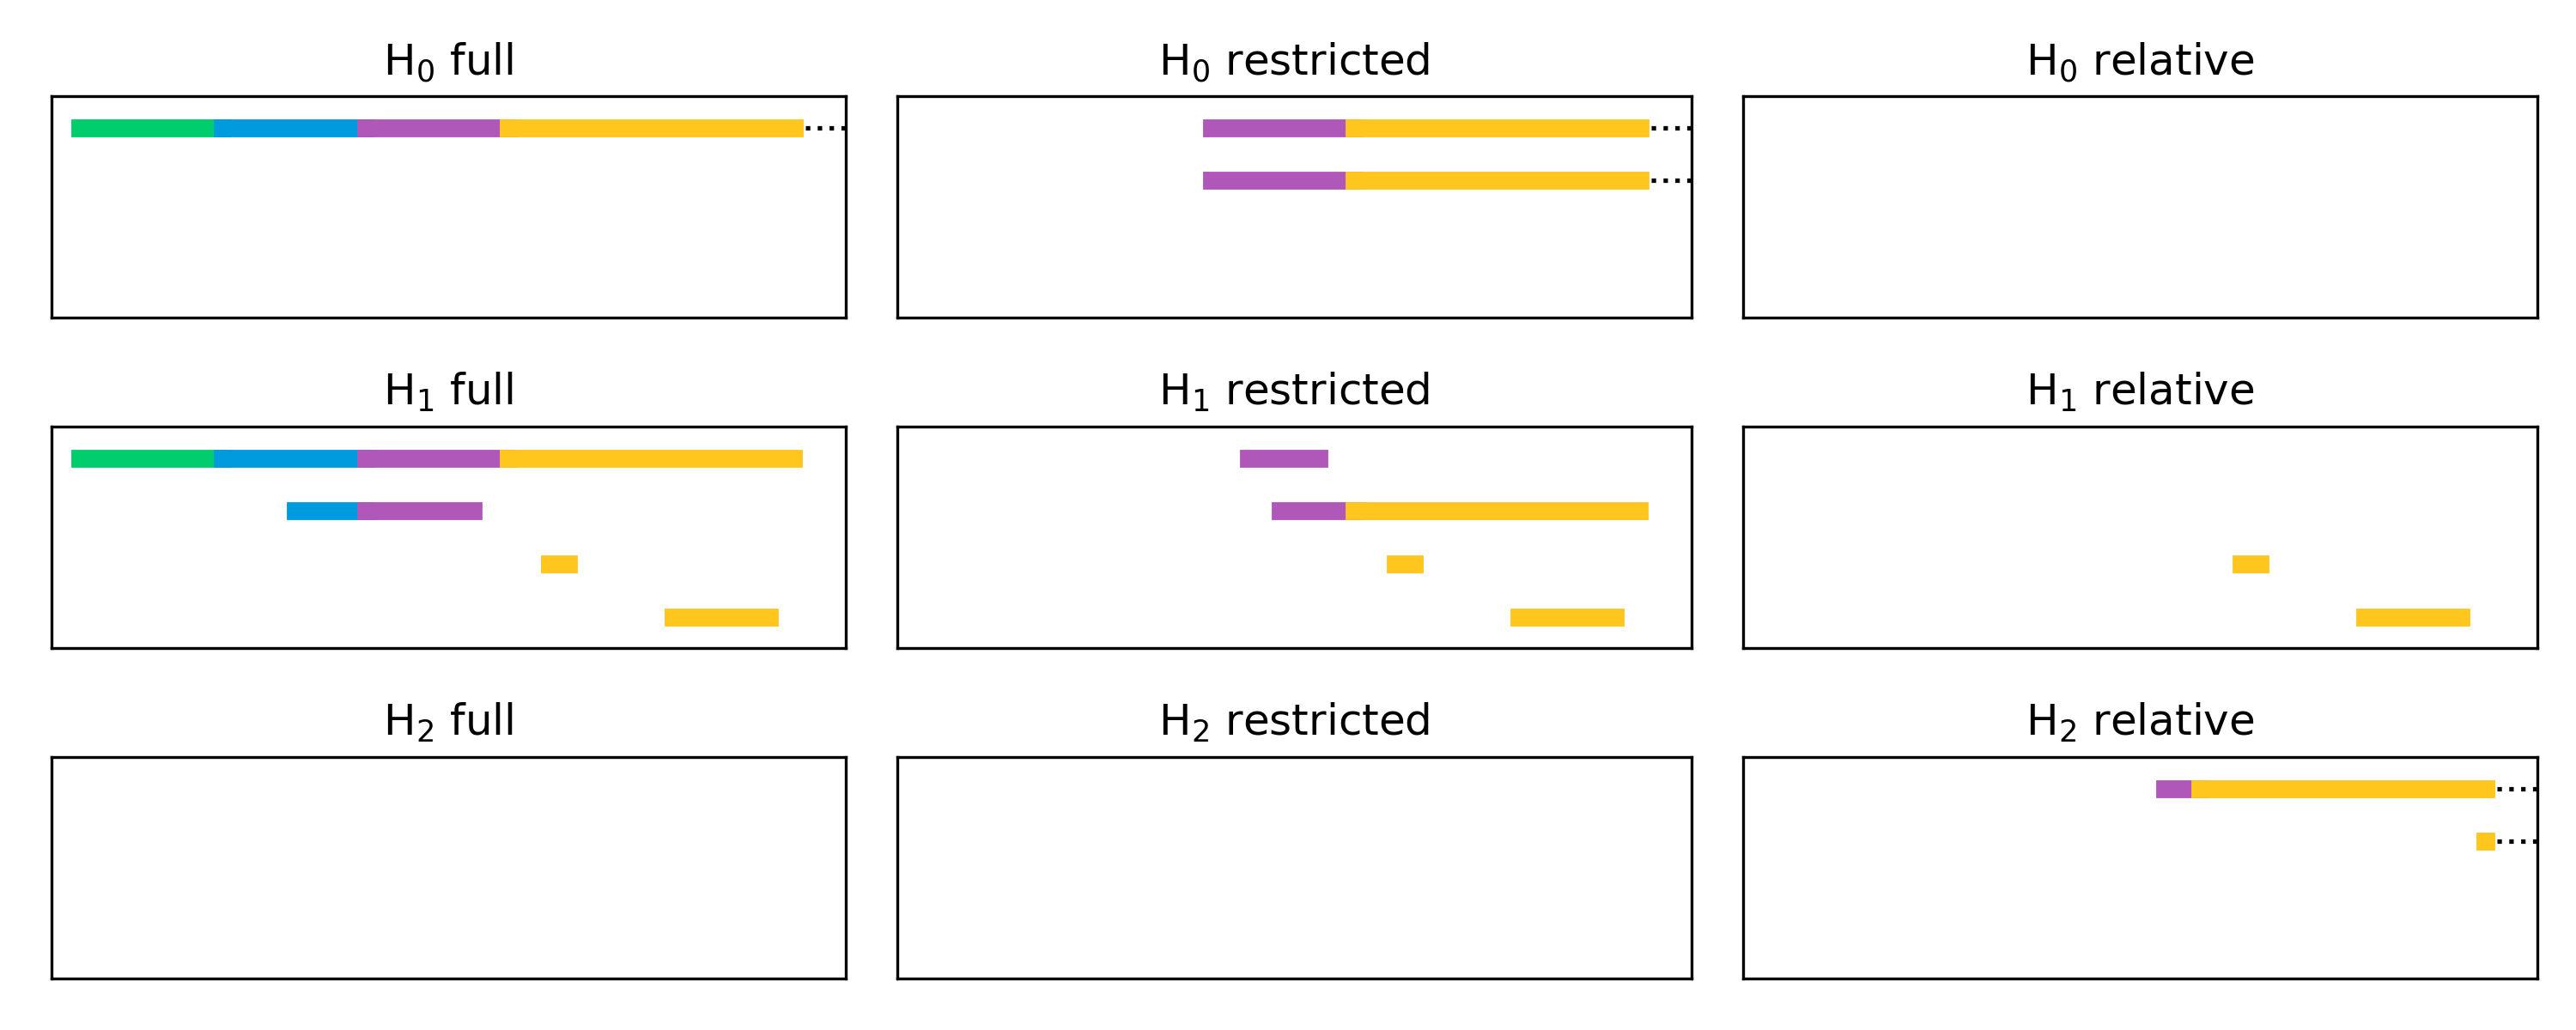
\includegraphics[width=\textwidth]{figures/barcode-res_rel.png}
  \end{minipage}
  \caption{Full, restricted, and relative barcodes of the function (left).}
\end{figure}

Let $\LL^k$ denote the $k$th persistent homology module of the sublevel set filtration $\{B_\alpha\}_{\alpha\in\R}$.
As in the previous section, let $\DD{\omega}^k$ denote the $k$th persistent (relative) homology module of $\{(D\subi{\omega}{\alpha}, B_\omega)\}_{\alpha\in\R}$.
Throughout we will assume that we are taking homology in a field $\FF$ and that the homology groups $\hom_k(B_\alpha)$ and $\hom_k(D\subi{\omega}{\alpha}, B_\omega)$ are finite dimensional vector spaces for all $k$ and $\alpha\in\R$.
We will use the interval decomposition of $\LL^k$ to give a decomposition of the relative module $\DD{\omega}^k$ in terms of a \emph{truncation} of $\LL^k$.
For fixed $\omega\in\R$ we will define the truncation $\T^k_\omega$ of $\LL^k$ in terms of the intervals decomposing $\LL^k$ that are in $[\omega, \infty)$.

\paragraph*{Truncated Interval Modules}

For an interval $I = [s,t)\subseteq \R$ let $I_+ := [t,\infty)$ and $I_- := (-\infty, s]$.
For $\omega\in\R$ let $\FF_{\omega}^I$ denote the interval module consisting of vector spaces $\{F\subi{\omega}{\alpha}^I\}_{\alpha\in\R}$ and linear maps $\{f\subi{\omega}{\alpha,\beta}^I : F\subi{\omega}{\alpha}^I\to F\subi{\omega}{\beta}^I\}_{\alpha\leq\beta}$ where
\[ F\subi{\omega}{\alpha}^I := \begin{cases} F_\alpha^I&\text{ if } \omega\in I_-\\ 0&\text{ otherwise,}\end{cases}\ \text{ and }\ \ f\subi{\omega}{\alpha,\beta}^I := \begin{cases} f_{\alpha,\beta}^I&\text{ if } \omega\in I_-\\ 0&\text{ otherwise.}\end{cases}\]
For a collection $\I$ of intervals let $\I_\omega := \{I\in\I\mid \omega\in I\}$.

\begin{lemma}\label{lem:decomposition}
  Suppose $\I^k$ and $\I^{k-1}$ are collections of intervals that decompose $\LL^k$ and $\LL^{k-1}$, respectively.
  Then for all $k$ the $k$th persistent homology module of $\{(D\subi{\omega}{\alpha}, B_\omega)\}_{\alpha\in\R}$ is isomorphic to
  \[\bigoplus_{I\in\I^k} \FF_\omega^I \oplus \bigoplus_{I\in \I_\omega^{k-1}} \FF^{I_+}.\]
\end{lemma}
\begin{proof}
  Suppose $\alpha\leq\omega$.
  So $\hom_k(D\subi{\omega}{\alpha}, B_\omega) = 0$ as $D\subi{\omega}{\alpha} = B_\omega\cup B_\alpha$ and $\T^k_\omega = 0$ as $F_\alpha^I = 0$ for any $I\in \I^k$ such that $\omega\in I_-$.
  Moreover, $\omega\in I$ for all $I\in \I_\omega^{k-1}$, thus $F_\alpha^{I_+} = 0$ for all $\alpha\leq\omega$.
  So it suffices to assume $\omega < \alpha$.

  Consider the long exact sequence of the pair $\hom_k(D\subi{\omega}{\alpha}, B_\omega) = \hom_k(B_\alpha, B_\omega)$
  \[ \ldots\to \hom_k(B_\omega)\xrightarrow{p_\alpha^k} \hom_k(B_\alpha)\xrightarrow{q_\alpha^k}\hom_k(D\subi{\omega}{\alpha}, B_\omega)\xrightarrow{r_\alpha^k} \hom_{k-1}(B_\omega)\xrightarrow{p_\alpha^{k-1}}\hom_{k-1}(B_\alpha)\to\ldots\]
  where $\hom_k(B_\alpha) = \bigoplus_{I\in \I^k}F_\alpha^I$, $\hom_k(B_\omega) = \bigoplus_{I\in \I^k}F_\omega^I$, and $p_\alpha^k = \displaystyle\bigoplus_{I\in\I^k} f_{\omega,\alpha}^I$.

  Noting that $\im~q_\alpha^k \cong \hom_k(B_\alpha) / \ker~q_\alpha^k$ where $\ker~q_\alpha^k = \im~p_\alpha^k$ by exactness we have $\ker~r_\alpha^k \cong \hom_k(B_\alpha) / \im~p_\alpha^k$.
  By the definition of $F_\alpha^I$ and $f_{\omega,\alpha}^I$ we know $\im~f_{\omega,\alpha}^I$ is $F_\alpha^I$ if $\omega\in I$ and 0 otherwise.
  As $\im~p_\alpha^k$ is equal to the direct sum of images $\im~f_{\omega,\alpha}^I$ over $I\in\I^k$ it follows that $\im~p_\alpha^k$ is the direct sum of those $F_\alpha^I$ over those $I\in\I^k$ such that $\omega\in I$.
  Now, because $\hom_k(B_\alpha) = \bigoplus_{I\in \I^k}F_\alpha^I$ and each $F_\alpha^I$ is either 0 or $\FF$ the quotient $\hom_k(B_\alpha) / \im~p_\alpha^k$ is the direct sum of those $F_\alpha^I$ such that $\omega\notin I$.
  Therefore, by the definition of $F\subi{\omega}{\alpha}^I$ we have
  \[ \ker~r_\alpha^k = \bigoplus_{I\in\I_\omega^k} F\subi{\omega}{\alpha}^I.\]

  Similarly, $\im~r_\alpha^k = \ker~p_\alpha^{k-1}$ by exactness where $\ker~p_\alpha^{k-1}$ is the direct sum of kernels $\ker~f_{\omega,\alpha}^I$ over $I\in\I^{k-1}$.
  By the definition of $F_\alpha^I$ and $f_{\omega,\alpha}^I$ we know that $\ker~f_{\omega,\alpha}^I$ is $F_\alpha^I$ if $\omega\notin I$ and $0$ otherwise.
  Noting that $\ker~f_{\omega,\alpha}^I = 0$ for any $I\in \I^{k-1}$ such that $\omega\notin I$ it suffices to consider only those $I\in \I_\omega^{k-1}$.
  It follows that $\ker~f_{\omega,\alpha}^I = F_\alpha^{I_+}$ for any $I$ containing $\omega$ as $\omega < \alpha$.
  Therefore,
  \[\im~r_\alpha^k = \bigoplus_{I\in\I^{k-1}} F_\alpha^{I_+}.\]

  We have the following split exact sequence associated with $r_\alpha^k$
  \[ 0\to \ker~r_\alpha^k\to \hom_k(D\subi{\omega}{\alpha}, B_\omega)\to\im~r_\alpha^k\to 0.\]
  The desired result follows from the fact that for all $\alpha\in\R$
  \begin{align*}
    \hom_k(D\subi{\omega}{\alpha}, B_\omega) &\cong \ker~r_\alpha^k\oplus \im~r_\alpha^k =\bigoplus_{I\in\I^k} F\subi{\omega}{\alpha}^I\oplus \bigoplus_{I\in\I_\omega^{k-1}} F_\alpha^{I_+}.
  \end{align*}
\end{proof}

Letting $\I^k$ denote the decomposing intervals of $\LL^k$ for all $k$ we can define the \textbf{$\omega$-truncated $k$th persistent homology module} of $\LL^k$ as
\[ \T_\omega^k := \bigoplus_{I\in\I^k} \FF_\omega^I\ \text{ and let }\ \LL_\omega^{k-1} := \bigoplus_{I\in \I_\omega^{k-1}} \FF^{I_+}\]
denote the submodule of $\DD{\omega}^k$ consisting of intervals $[\beta,\infty)$ corresponding to features $[\alpha,\beta)$ in $\LL^{k-1}$ such that $\alpha\leq\omega <\beta$.
Now, by Lemma~\ref{lem:decomposition} the $k$th persistent (relative) homology module of $\{(D\subi{\omega}{\alpha}, B_\omega)\}_{\alpha\in\R}$ is $\DD{\omega}^k = \T_\omega^k\oplus \LL_\omega^{k-1}.$
Theorems~\ref{thm:algo_tcc} and~\ref{thm:interleaving_main_2} can then be used to show that
\[ \{\rips^{2\delta}(P\subi{\omega-2c\delta}{\alpha}, Q_{\omega-2c\delta})\hookrightarrow \rips^{4\delta}(P\subi{\omega+c\delta}{\alpha}, Q_{\omega+c\delta})\}_{\alpha\in\R} \]
is $4c\delta$ interleaved with $\T_\omega^k\oplus \LL_\omega^{k-1}$ whenever
\[ \rk~\hom_d(\rips^\delta(P, Q_{\omega - 2c\delta})\hookrightarrow \rips^{2\delta}(P, Q_{\omega+c\delta})) \geq \dim~\hom_0(\rips^\delta(P\setminus Q_{\omega-2c\delta})).\]


%   If $\rk~\hom_d(\rips^\delta(P, Q_{\omega - 2c\delta})\hookrightarrow \rips^{2\delta}(P, Q_{\omega+c\delta})) \geq \dim~\hom_0(\rips^\delta(P\setminus Q_{\omega-2c\delta}))$ then the $k$th (relative) homology module of $\{\rips^{2\delta}(P\subi{\omega-2c\delta}{\alpha}, Q_{\omega-2c\delta})\hookrightarrow \rips^{4\delta}(P\subi{\omega+c\delta}{\alpha}, Q_{\omega+c\delta})\}_{\alpha\in\R}$ is $4c\delta$-interleaved with $\T_{\omega}^k \oplus \LL_\omega^{k-1}$: the $k$th persistent homology module of $\{(D\subi{\omega}{\alpha}, B_\omega)\}_{\alpha\in\R}$.
%
% Our main theorem combines this decomposition with our coverage and interleaving results of Theorems~\ref{thm:algo_tcc} and~\ref{thm:interleaving_main_2}.% as a method for certified approximation of the truncated persistence diagram.\textbf{TODO: GROSS}

% \begin{lemma}\label{lem:dual_ass}
%   Let $\X$ be an orientable $d$-manifold and suppose $(D, B)$ and $(D, B')$ are compact, locally contractible, surrounding pairs in $\X$ such that $\hom_d(D, B)$ and $\hom_d(D, B')$ are finitely generated.
%
%   If $\hom_{d-1}(B\hookrightarrow B')$ is surjective then $\hom_0(D\setminus B'\hookrightarrow D\setminus B)$ is injective.
%   If $\hom_{d-1}(B\hookrightarrow B')$ is injective then $\hom_0(D\setminus B'\hookrightarrow D\setminus B)$ is surjective.
% \end{lemma}
% \begin{proof}
%   If $\hom_{d-1}(B\hookrightarrow B')$ is surjective for all $k$ then $\hom_d((D, B)\hookrightarrow (D, B'))$ is surjective by the five lemma.
%   Taking homology with coefficients in a field $\FF$ we can dualize to obtain an \emph{injective} map $\Hom(\hom_d(D,B'), \FF)\to \Hom(\hom_d(D, B), \FF)$.
%   Therefore, because we are taking coefficients in a field, we have an injective map $\hom^d(D,B')\to \hom^d(D, B)$ by the Universal Coefficient Theorem.
%
%   Because $(D, B)$ and $(D,B')$ are compact and locally connected we can apply Alexander Duality to obtain an injective map $\hom_0(\X\setminus B', \X\setminus D)\to\hom_0(\X\setminus B, \X\setminus D)$.
%   Because $B,B'$ surround $D$ in $\X$ it follows that $\hom_0(D\setminus B'\hookrightarrow D\setminus B)$ is injective.
%   It can be shown $\hom_{d-1}(B\hookrightarrow B')$ injective implies $\hom_0(D\setminus B'\hookrightarrow D\setminus B)$ surjective by a similar argument.
% \end{proof}
%
% \begin{theorem}\label{thm:main}
%   Let $\X$ be an orientable $d$-manifold and let $D$ be a compact subset of $\X$.
%   Let $f : D\to\R$ be a $c$-Lipschitz function and $\omega\in\R$, $\delta < \varrho_D/4$ be constants such that $P\subset D$ is a $(\delta, 2\delta,\omega)$-sublevel sample of $f$ and $B_{\omega-3c\delta}$ surrounds $D$ in $\X$.
%   % Let $P$ be a finite subset of $D$ such that $(P, Q_{\omega-2c\delta})$ and $(P, Q_{\omega+c\delta})$ are $\delta$-good samples of $(D, B_\omega)$.
%   % Let $P\subset \intr_\X(D)$ and suppose $D\setminus P^\delta$, $D\setminus Q_{\omega-2c\delta}^\delta$, and $D\setminus Q_{\omega+c\delta}^\delta$ are locally path connected.
%
%   Suppose $\hom_k(B_{\omega-3c\delta}\hookrightarrow B_\omega)$ is surjective and $\hom_k(B_\omega\hookrightarrow B_{\omega+5c\delta})$ is an isomorphism for all $k$.
%   If $\rk~\hom_d(\rips^\delta(P, Q_{\omega - 2c\delta})\hookrightarrow \rips^{2\delta}(P, Q_{\omega+c\delta})) \geq \dim~\hom_0(\rips^\delta(P\setminus Q_{\omega-2c\delta}))$ then the $k$th (relative) homology module of $\{\rips^{2\delta}(P\subi{\omega-2c\delta}{\alpha}, Q_{\omega-2c\delta})\hookrightarrow \rips^{4\delta}(P\subi{\omega+c\delta}{\alpha}, Q_{\omega+c\delta})\}_{\alpha\in\R}$ is $4c\delta$-interleaved with $\T_{\omega}^k \oplus \LL_\omega^{k-1}$: the $k$th persistent homology module of $\{(D\subi{\omega}{\alpha}, B_\omega)\}_{\alpha\in\R}$.
%    % that of $\{(D\subi{\omega}{\alpha}, B_\omega)\}_{\alpha\in\R}$.
% \end{theorem}
% \begin{proof}
%   If $\hom_k(B_{\omega-3c\delta}\hookrightarrow B_\omega)$ is surjective for all $k$ then, in particular, $\hom_{d-1}(B_{\omega-3c\delta}\hookrightarrow B_\omega)$ is surjective.
%   If $\hom_k(B_{\omega-3c\delta}\hookrightarrow B_\omega)$ is surjective for all $k$ then, in particular, $\hom_{d-1}(B_{\omega-3c\delta}\hookrightarrow B_\omega)$ is surjective.
%   Because $B_{\omega-3c\delta}, B_\omega$ are closed in $D$, and $D$ is compact, $(D, B_{\omega-3c\delta})$ and $(D,B_\omega)$ are compact pairs.
%   If our pairs are locally contractible then $\hom_0(D\setminus B_\omega\hookrightarrow D\setminus B_{\omega-3c\delta})$ is injective and $\hom_0(D\setminus B_{\omega-5c\delta}\hookrightarrow D\setminus B_\omega)$ is surjective by Lemma~\ref{lem:dual_ass}.
%
%   Because $\rk~\hom_d(\rips^\delta(P, Q_{\omega - 2c\delta})\hookrightarrow \rips^{2\delta}(P, Q_{\omega+c\delta})) \geq \dim~\hom_0(\rips^\delta(P\setminus Q_{\omega-2c\delta}))$ and $P\subset D$ is a $(\delta, 2\delta,\omega)$-sublevel sample of $f$ we have $D\setminus B_\omega\subseteq P^\delta$ and $Q_{\omega-2c\delta}^\delta$ surrounds $P^\delta$ in $D$ by Theorem~\ref{thm:algo_tcc}.
%   So the persistent homology modules of $\{\rips^{2\delta}(P\subi{\omega-2c\delta}{\alpha}, Q_{\omega-2c\delta})\hookrightarrow \rips^{4\delta}(P\subi{\omega+c\delta}{\alpha}, Q_{\omega+c\delta})\}_{\alpha\in\R}$ are $4c\delta$ interleaved with those of $\{(D\subi{\omega}{\alpha}, B_\omega)\}_{\alpha\in\R}$ by Theorem~\ref{thm:interleaving_main_2}, and therefore $\T_{\omega}^k \oplus \LL_\omega^{k-1}$ by Lemma~\ref{lem:decomposition}.
% \end{proof}
